\section{\label{sec:convention}Conventions for representing space groups}

\subsection{Conventional cell}

% Primitive basis and primitive cell
It is natural to choose a basis for a translation lattice of a space group such that all symmetry operations are represented by integer matrices.
Such a basis is called a \term{primitive basis} of the lattice, and a unit cell spanned by the primitive basis is called a \term{primitive cell}.

% Centered basis and conventional cell
Although the primitive basis is useful for mathematical and algorithmic treatments, we often use a non-primitive basis, called a \term{centered basis}, to represent the lattice for humans.
There are conventions on which centered basis to choose for each lattice system, which is called a \term{conventional basis} \cite{burzlaff2016crystal}.
A unit cell spanned by the conventional basis is called a \term{conventional cell}.
The conventional bases are chosen as right-handed with the following rules:

\paragraph{Triclinic lattice system ($aP$)}
Choose the Niggli reduced basis \cite{Krivy:a12875}.

\paragraph{Monoclinic lattice system ($mP, mS$)}
The only symmetry direction is labeled $\bm{b}$.
The other basis vectors $\bm{a}$ and $\bm{c}$ are chosen to be the shortest two vectors perpendicular to $\bm{b}$ with a non-acute angle.
The other settings to choose $\bm{a}$ or $\bm{c}$ as the unique axis are also used.

\paragraph{Orthorhombic lattice system ($oP, oS, oF, oI$)}
Choose basis vectors along the three twofold axes.

\paragraph{Tetragonal lattice system ($tP, tI$)}
The vector $\bm{c}$ is along the fourfold axis.
The $\bm{a}$ and $\bm{c}$ are chosen along the twofold axes perpendicular to each other.

\paragraph{Rhombohedral lattice system ($hR$)}
There are two descriptions in ITA~\cite{ITA2016}, \term{hexagonal axes} and \term{rhombohedral axes}.
For the hexagonal axes, the vector $\bm{c}$ is parallel to the threefold axis;
The $\bm{a}$ and $\bm{b}$ are chosen along twofold axes perpendicular to $\bm{c}$ with angle of $120^{\circ}$ so that lattice points occur at $2/3, 1/3, 1/3$ and $1/3, 2/3, 2/3$ (\term{obverse} setting).
The \term{reverse} setting with lattice points $1/3, 2/3, 1/3$ and $2/3, 1/3, 2/3$ is not used.
For the rhombohedral axes, choose the shortest three lattice vectors equivalent to the threefold axis.
See Fig~\ref{fig:hexagonal_axes} for the projections along $c$ of rhombohedral and hexagonal axes.

\begin{figure}[htb]
  \centering
  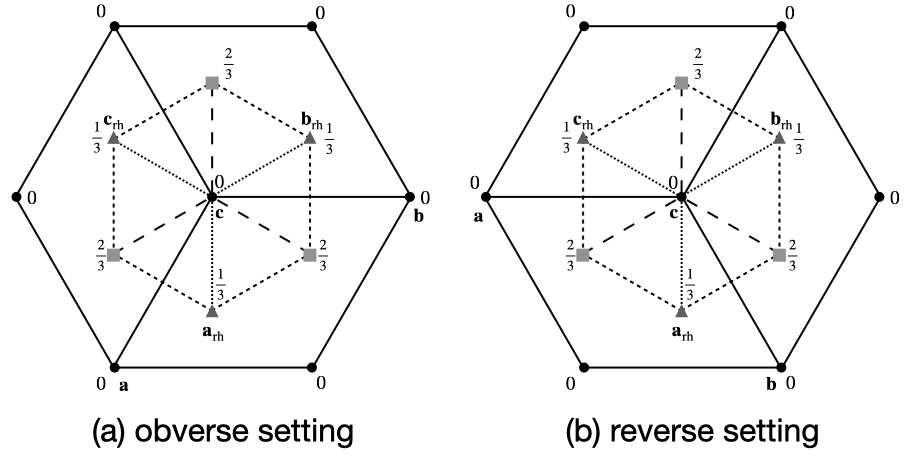
\includegraphics[width=0.9\textwidth]{figure/fig_hexagonal_axes.png}
  \caption{Projections of hexagonal axes of rhombohedral lattice in (a) obverse and (b) reserve settings.}
  \label{fig:hexagonal_axes}
\end{figure}

\paragraph{Hexagonal lattice system ($hP$)}
The vector $\bm{c}$ is parallel to the sixfold axis.
The $\bm{a}$ and $\bm{b}$ are chosen along twofold axes perpendicular to $\bm{c}$ with angle of $120^{\circ}$.

\paragraph{Cubic lattice system ($cP, cF, cI$)}
Choose basis vectors parallel to the fourfold axes.

\subsection{Hermann--Mauguin symbol}

The Hermann--Mauguin (HM) symbols represent space groups concisely.
The first constituent of the HM symbol characterizes the conventional cell of the translation lattice, one of $P, A, B, C, F, I$, and $R$.
The remained constituents describe generators of the space group.

One way to read the HM symbols is as follows (along with the example $Cmc2_{1}$):
\begin{enumerate}
  \item Read the conventional cell from the first constituent (base-centered basis $C$)
  \item Determine the geometric crystal class by ignoring translation parts ($mm2$)
  \item Determine the crystal class ($mm2 \, \rightarrow \, \mbox{orthorhombic}$)
  \item Read symmetry directions from Table~\ref{tab:hermann-mauguin}
\end{enumerate}

\begin{table}[htb]
  \caption{Symmetry directions for the short Hermann--Mauguin symbols in space groups}
  \label{tab:hermann-mauguin}
  \centering
  \begin{tabular}{cccc}
    \hline\hline
    Crystal system & Primary & Secondary & Tertiary  \\ \hline
    Triclinic                         & None  & & \\
    Monoclinic (unique axis $\bm{b}$) & [010] & & \\
    Orthorhombic                      & [100] & [010] & [001] \\
    Tetragonal                        & [001] & $\langle 100 \rangle$ & $\langle 1\overline{1}0 \rangle $ \\
    Trigonal ($P$ lattice) & [001] & $\langle 100 \rangle$ & None \\
                           & [001] & None & $\langle 1\overline{1}0 \rangle $ \\
    Trigonal ($R$ lattice, hexagonal axes) &
      $[001]_{\mathrm{hex}}$ & $\langle 100 \rangle_{\mathrm{hex}}$ & \\
    Trigonal ($R$ lattice, rhombohedral axes) &
      $[111]_{\mathrm{rhomb}}$ & $\langle 1\overline{1}0 \rangle_{\mathrm{rhomb}}$ & \\
    Hexagonal                        & [001] & $\langle 100 \rangle$ & $\langle 1\overline{1}0 \rangle$ \\
    Cubic                            & $\langle 001 \rangle$ & $\langle 111 \rangle$ & $\langle 1\overline{1}0 \rangle$ \\
    \hline\hline
  \end{tabular}
\end{table}

% The number of generators of space groups can be chosen as at most three.

\subsection{Conventional descriptions of space group types in ITA}

ITA provides several descriptions for some of the space-group types.

\subsubsection{Setting and cell choice for monoclinic crystal system}

% See Sec.~2.1.3.15 of Ref.~\cite{ITA2016} for more details.
For monoclinic space groups, ITA gives two options to describe the space groups, \term{setting} (\term{unique axis}) and \term{cell choice}.
The setting refers to the assignment of labels $a$, $b$, and $c$, which describes which basis vectors directs to the unique symmetry direction.
After determining the unique axis, there are three possibilities to take the remaining shortest basis vectors perpendicular to the unique axis with a non-acute angle.
The cell choice refers to the assignment out of the three cell choices.
See Fig.~\ref{fig:monoclinic-choices} for combinations of settings and cell choices for monoclinic-centered lattices.

\begin{figure}[htb]
  \centering
  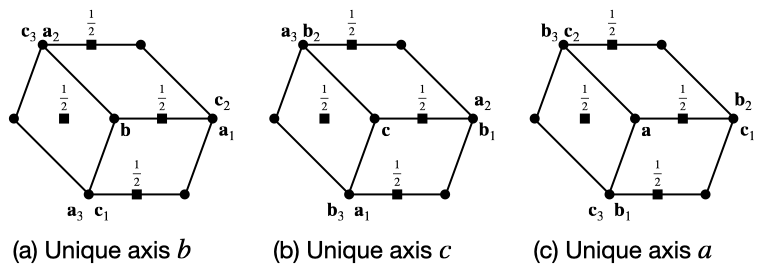
\includegraphics[width=\textwidth]{figure/fig_monoclinic_settings_cell_choices.png}
  \caption{
    Monoclinic-centered lattices.
    (a) Unique axis $b$:
      cell choice 1 ($C$-centered cell with $\bm{a}_{1}, \bm{b}, \bm{c}_{1}$),
      cell choice 2 ($A$-centered cell with $\bm{a}_{2}, \bm{b}, \bm{c}_{2}$),
      cell choice 3 ($I$-centered cell with $\bm{a}_{3}, \bm{b}, \bm{c}_{3}$).
    (b) Unique axis $c$:
      cell choice 1 ($A$-centered cell with $\bm{a}_{1}, \bm{b}, \bm{c}_{1}$),
      cell choice 2 ($B$-centered cell with $\bm{a}_{2}, \bm{b}, \bm{c}_{2}$),
      cell choice 3 ($I$-centered cell with $\bm{a}_{3}, \bm{b}, \bm{c}_{3}$).
    (c) Unique axis $a$:
      cell choice 1 ($B$-centered cell with $\bm{a}_{1}, \bm{b}, \bm{c}_{1}$),
      cell choice 2 ($C$-centered cell with $\bm{a}_{2}, \bm{b}, \bm{c}_{2}$),
      cell choice 3 ($I$-centered cell with $\bm{a}_{3}, \bm{b}, \bm{c}_{3}$).
  }
  \label{fig:monoclinic-choices}
\end{figure}

The unique axis $b$ setting with cell choice 1 is standard for monoclinic space groups.
The transformation matrices to the unique axis $b$ are shown in Table~\ref{tab:monoclinic-settings}.
For the unique axis $b$, the transformation matrices to cell choice 1 are shown in Table~\ref{tab:monoclinic-cell-choice}.

\begin{table}[htb]
  \centering
  \small
  \caption{Transformation matrices to unique axis $b$ for monoclinic space groups.}
  \label{tab:monoclinic-settings}
  \begin{tabular}{c|ccc}
    \hline\hline
    Setting (unique axis) & $b$ & $c$ & $a$ \\
    \hline
    Transformation to unique axis $b$ &
      $\begin{pmatrix} 1& 0&0 \\ 0& 1&0 \\ 0& 0&1 \end{pmatrix}$ &
      $\begin{pmatrix}0& 0&1 \\1& 0&0 \\0& 1&0\end{pmatrix}$ &
      $\begin{pmatrix} 0&1&0 \\ 0&0&1 \\ 1&0&0 \end{pmatrix}$ \\
    Cell choice 1 & $C \to C$ & $A \to C$ & $B \to C$ \\
    Cell choice 2 & $A \to A$ & $B \to A$ & $C \to A$ \\
    Cell choice 3 & $I \to I$ & $I \to I$ & $I \to I$ \\
    \hline\hline
  \end{tabular}
\end{table}

\begin{table}[htb]
  \centering
  \caption{Transformation matrices to cell choice 1 for monoclinic space groups with the unique axis $b$.}
  \label{tab:monoclinic-cell-choice}
  \begin{tabular}{c|ccc}
    \hline\hline
    Cell choice & 1 & 2 & 3 \\
    \hline
    Transformation to cell choice 1
      & $\begin{pmatrix} 1&0&0\\0&1&0\\0&0&1 \end{pmatrix}$
      & $\begin{pmatrix} -1&0&1\\0&1&0\\-1&0&0 \end{pmatrix}$
      & $\begin{pmatrix} 0&0&-1\\0&1&0\\1&0&-1 \end{pmatrix}$ \\
    Centering & $C \to C$ & $A \to C$ & $I \to C$ \\
    \hline\hline
  \end{tabular}
\end{table}

\subsubsection{Setting for orthorhombic crystal system}

For a conventional basis $\bm{a}$, $\bm{b}$, and $\bm{c}$ of an orthorhombic crystal system, ITA gives the following six permutations of axes,
\begin{align*}
  \mathbf{abc}, \mathbf{ba\overline{c}}, \mathbf{cab}, \mathbf{\overline{c}ba}, \mathbf{bca}, \mathbf{a\overline{c}b},
\end{align*}
where the overline (e.g. $\mathbf{\overline{a}}$) indicates the negative direction.
The transformation matrices from each setting to $\mathbf{abc}$ are shown in Table~\ref{tab:orthorhombic-settings}.

\begin{table}[htb]
  \centering
  \small
  \caption{Transformation matrices to $\mathbf{abc}$ for orthorhombic space groups.}
  \label{tab:orthorhombic-settings}
  \begin{tabular}{ccc}
    \hline\hline
    Setting & Transformation to $\mathbf{abc}$ & Centering \\
    \hline
    $\mathbf{abc}$
       & $\begin{pmatrix} 1& 0&0 \\ 0& 1&0 \\ 0& 0&1 \end{pmatrix}$
       & $A \to A, B \to B, C \to C$ \\
    $\mathbf{ba\overline{c}}$
      & $\begin{pmatrix} 0&1&0 \\ 1&0&0 \\ 0&0&-1 \end{pmatrix}$
      & $A \to B, B \to A, C \to C$ \\
    $\mathbf{cab}$
      & $\begin{pmatrix}0& 0&1 \\1& 0&0 \\0& 1&0\end{pmatrix}$
      & $A \to C, B \to A, C \to B$ \\
    $\mathbf{\overline{c}ba}$
      & $\begin{pmatrix} 0&0&-1 \\ 0&1&0 \\ 1&0&0 \end{pmatrix}$
      & $A \to C, B \to B, C \to A$ \\
    $\mathbf{bca}$
      & $\begin{pmatrix} 0&1&0 \\ 0&0&1 \\ 1&0&0 \end{pmatrix}$
      & $A \to B, B \to C, C \to A$ \\
    $\mathbf{a\overline{c}b}$
      & $\begin{pmatrix} 1&0&0 \\ 0&0&-1 \\ 0&1&0 \end{pmatrix}$
      & $A \to A, B \to C, C \to B$ \\
    \hline\hline
  \end{tabular}
\end{table}

\subsubsection{Origin choice for centrosymmetric groups}

We refer to space groups with an inversion symmetry as \term{centrosymmetric}.
Otherwise, we call space groups without an inversion symmetry as \term{noncentrosymmetric}.
For noncentrosymmetric space groups, the origin is chosen at a point of the highest site-symmetry as conventions.
For centrosymmetric space groups, ITA gives the two descriptions for the origins at
\begin{itemize}
  \item (Origin choice 1) a point of the highest site-symmetry;
  \item (Origin choice 2) an inversion center.
\end{itemize}
The origin choice 2 is standard for centrosymmetric space groups\footnote{
  Be careful \texttt{Spglib} chooses the origin choice 1 as default.
}.

\subsubsection{Hexagonal axes for rhombohedral space groups}

For rhombohedral space groups, ITA describes them with the (obverse) hexagonal axes and the rhombohedral axes.
The hexagonal axes are standard.
One of the transformation matrices from the rhombohedral cell to the obverse hexagonal cell is
\begin{align*}
  \begin{pmatrix}
    1 & 0 & 1 \\
    -1 & 1 & 1 \\
    0 & -1 & 1 \\
  \end{pmatrix},
\end{align*}
and its inverse transformation from the obverse hexagonal cell to the primitive rhombohedral cell is
\begin{align*}
  \begin{pmatrix}
    \frac{2}{3} & -\frac{1}{3} & -\frac{1}{3} \\
    \frac{1}{3} & \frac{1}{3} & -\frac{2}{3} \\
    \frac{1}{3} & \frac{1}{3} & \frac{1}{3} \\
  \end{pmatrix}.
\end{align*}

\subsubsection{Standard setting}

In summary, \href{https://www.cryst.ehu.es/cgi-bin/cryst/programs/nph-def-choice}{the standard setting} is one of the conventional descriptions for each space-group type used in the ITA \cite{ITA2016}: unique axis b setting, cell choice 1 for monoclinic space groups, hexagonal axes for rhombohedral space groups, and origin choice 2 for centrosymmetric space groups.

\subsection{Hall symbol}

Hall symbol \cite{Hall:a19707}

Computer adapted symbol
